%!TEX TS-program = xelatex
%!TEX encoding = UTF-8 Unicode

\documentclass[12pt]{extarticle}
% extarticle is like article but can handle 8pt, 9pt, 10pt, 11pt, 12pt, 14pt, 17pt, and 20pt text

\def \ititle {Origins of Mind}
 
\def \isubtitle {Lecture 08}
 
\def \iauthor {Stephen A. Butterfill}
\def \iemail{s.butterfill@warwick.ac.uk}
\date{}

%for strikethrough
\usepackage[normalem]{ulem}

\input{$HOME/Documents/submissions/preamble_steve_handout}

%logic symbol \leftmodels
\usepackage{MnSymbol}

%\bibpunct{}{}{,}{s}{}{,}  %use superscript TICS style bib
%remove hanging indent for TICS style bib
%TODO doesnt work
\setlength{\bibhang}{0em}
%\setlength{\bibsep}{0.5em}


%itemize bullet should be dash
\renewcommand{\labelitemi}{$-$}

\begin{document}

\raggedcolumns

\begin{multicols*}{3}

\setlength\footnotesep{1em}


\bibliographystyle{newapa} %apalike

%\maketitle
%\tableofcontents




%--------------- 
%--- start paste

\def \ititle {Logic I}
 
\def \isubtitle {Fast Lecture 06}
 
\begin{center}
 
{\Large
 
\textbf{\ititle}: \isubtitle
 
}
 
 
 
\iemail %
 
\end{center}
 
Readings refer to sections of the course textbook, \emph{Language, Proof and Logic}.
 
 
 
\section{Quantifier Equivalences: \\ ¬∀x Created(x) $\leftmodels\models$ ∃x ¬Created(x)}
 
\emph{Reading:} §10.1, §10.3, §10.4
 
 
 
\section{Proof Example: \\ ∃x Dead(x) $\vdash$ ¬∀x¬ Dead(x).}
 
\begin{center}
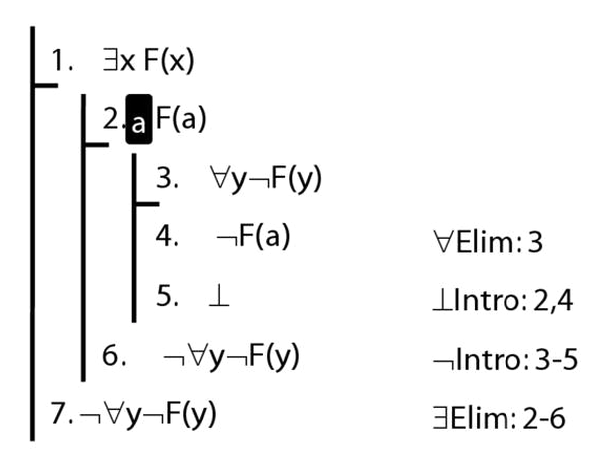
\includegraphics[scale=0.3]{img/unit_825_proof.png}
\end{center}
 
 
\section{Proof Example: \\ ¬∀x Dead(x) $\vdash$ ∃x¬ Dead(x).}
 
\begin{center}
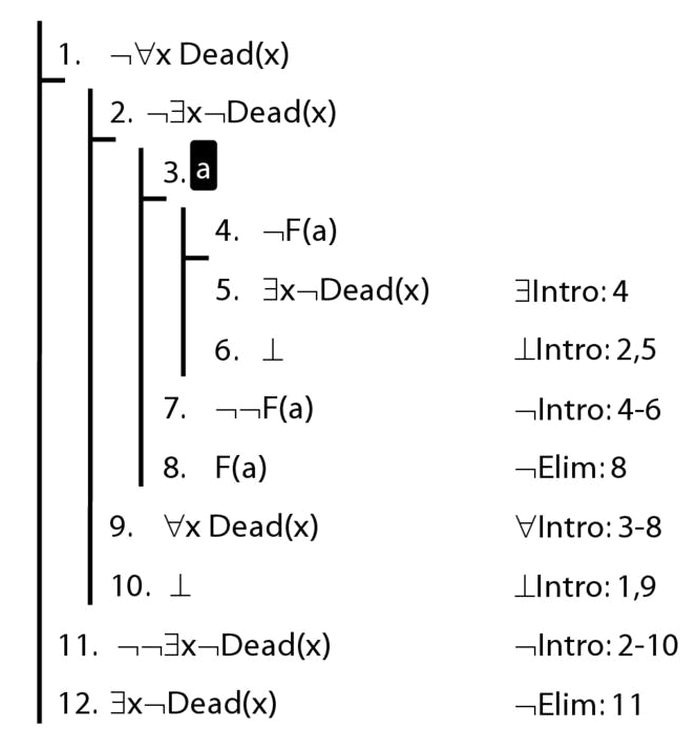
\includegraphics[scale=0.3]{img/unit_826_proof.png}
\end{center}
 
 
\section{Quantifier Equivalences: \\ ∀x(Square(x) → Broken(x)) \\ $\leftmodels\models$ ∀x(¬Broken(x) → ¬Square(x))}
 
\emph{Reading:} §10.3
 
\begin{center}
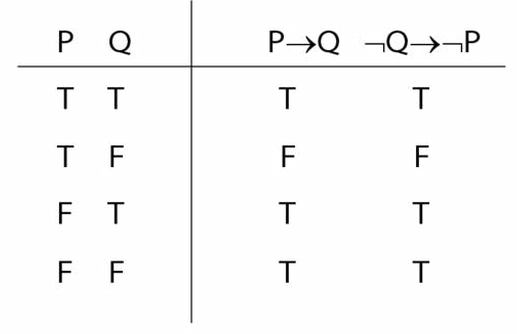
\includegraphics[scale=0.3]{img/unit_760_tt.png}
\end{center}
 
 
\section{There Does Not Exist}
 
Something is not dead:
 
\hspace{3mm} ∃x ¬Dead(x)
 
Nothing is dead:
 
\hspace{3mm} ¬∃x Dead(x)
 
Everything is not broken:
 
\hspace{3mm} ∀x ¬Broken(x)
 
Not everything is broken:
 
\hspace{3mm} ¬∀x Broken(x)
 
\begin{center}
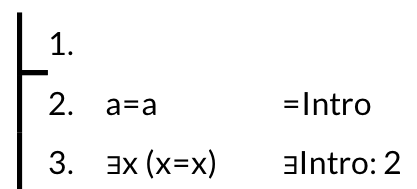
\includegraphics[scale=0.3]{img/unit_605_prf1.png}
\end{center}
\begin{center}
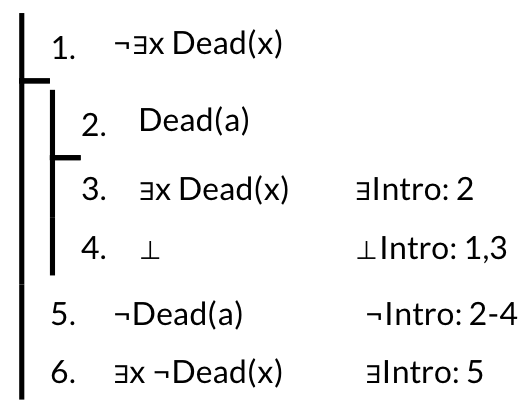
\includegraphics[scale=0.3]{img/unit_605_prf2.png}
\end{center}
\begin{center}
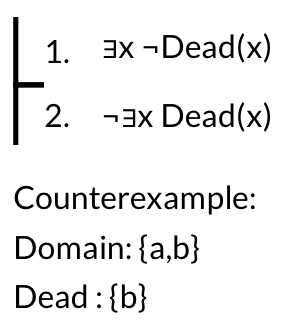
\includegraphics[scale=0.3]{img/unit_605_counterexample.png}
\end{center}
 
 
\section{Two Things Are Broken}
 
\emph{Reading:} §14.1
 
To translate sentences involving number into FOL, use identity. For example,
 
`Two things are broken' might be translated as:
 
∃x ∃y ( Broken(x) ∧ Broken(y) ∧ ¬(x=y) )
 
 
 
\section{There Is Exactly One}
 
There is one creator (at least one, maybe more).
 
∃x Creator(x)
 
Brian is the one and only creator.
 
Creator(b) ∧ ∀x( Creator(x) → x=b )
 
All squares are broken.
 
∀x( Sqr(x) → Brkn(x) )
 
There is one and only one creator.
 
∃y( Creator(y) ∧ ∀x( Creator(x) → x=y ) )
 
or:
 
∃y( ∀x( Creator(x) ↔ x=y ) )
 
 
 
\section{Variables}
 
Names : a, b, c, …
 
Variables : x, y, z, w, …
 
Variables are for saying several things about one thing even without specifying which thing it is
 
NB: `Some x is a horse and x is dead' ain't English.
 
 
 
\section{More Dead Horse}
 
\emph{Reading:} §11.4, §11.5
 
\begin{center}
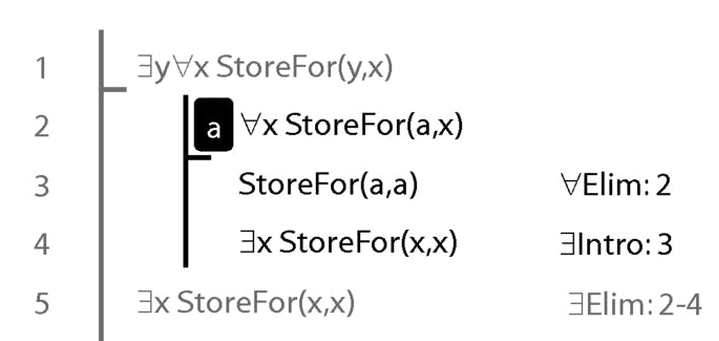
\includegraphics[scale=0.3]{img/unit_565_proof.png}
\end{center}
“Tesco is a store for everything”
 
∀x StoreFor(b,x)
 
Tesco is a store for everything except dead horses
 
∀x (¬DeadHorse(x) → StoreFor(b,x) )
 
Tesco is a store for everything except Tesco
 
∀x (¬x=b → StoreFor(b,x) )
 
There is a store for everything except itself
 
∃y ∀x (¬x=y → StoreFor(y,x) )
 
 
 
\section{↔ : truth tables and rules}
 
\begin{center}
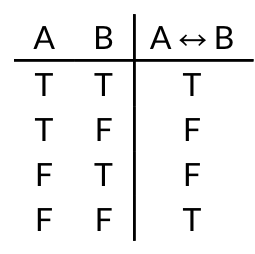
\includegraphics[scale=0.3]{img/tt_biconditional.png}
\end{center}
\begin{center}
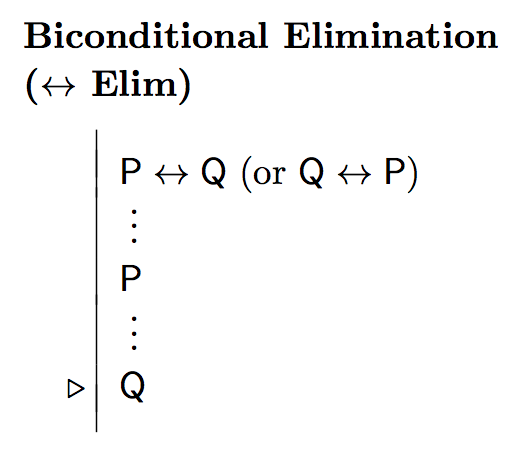
\includegraphics[scale=0.3]{img/rule_biconditional_elim.png}
\end{center}
\begin{center}
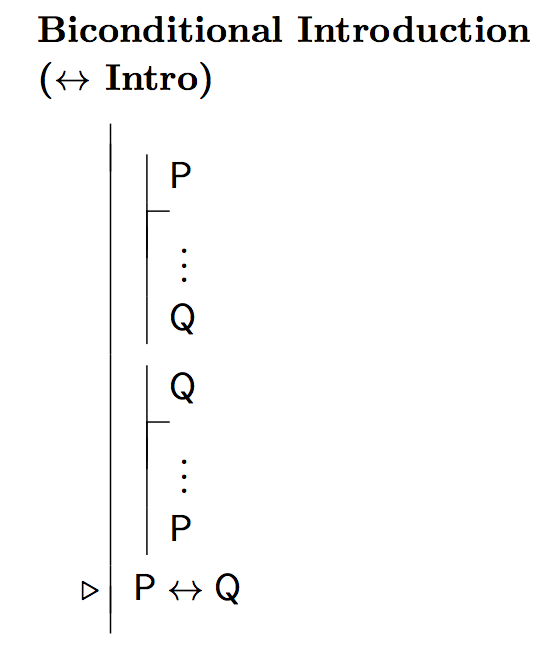
\includegraphics[scale=0.3]{img/rule_biconditional_intro.png}
\end{center}
 
 
\section{∀Intro: An Incorrect Proof}
 
\emph{Reading:} §13.1, §13.2
 
This proof is wrong, but why?:
 
\begin{center}
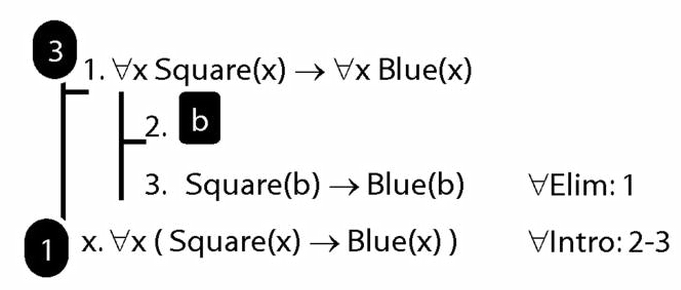
\includegraphics[scale=0.3]{img/unit_572_proof.png}
\end{center}
There is a counterexample to the argument:
 
\begin{center}
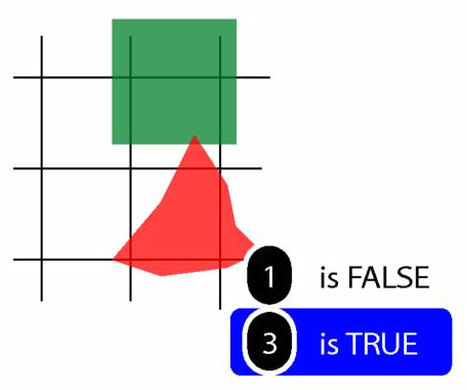
\includegraphics[scale=0.3]{img/unit_572_proof2.png}
\end{center}
 
 
\section{How Big Is a Truth-Table?}
 
How many truth-functions can be constructed using 2 sentence letters?
 
\begin{center}
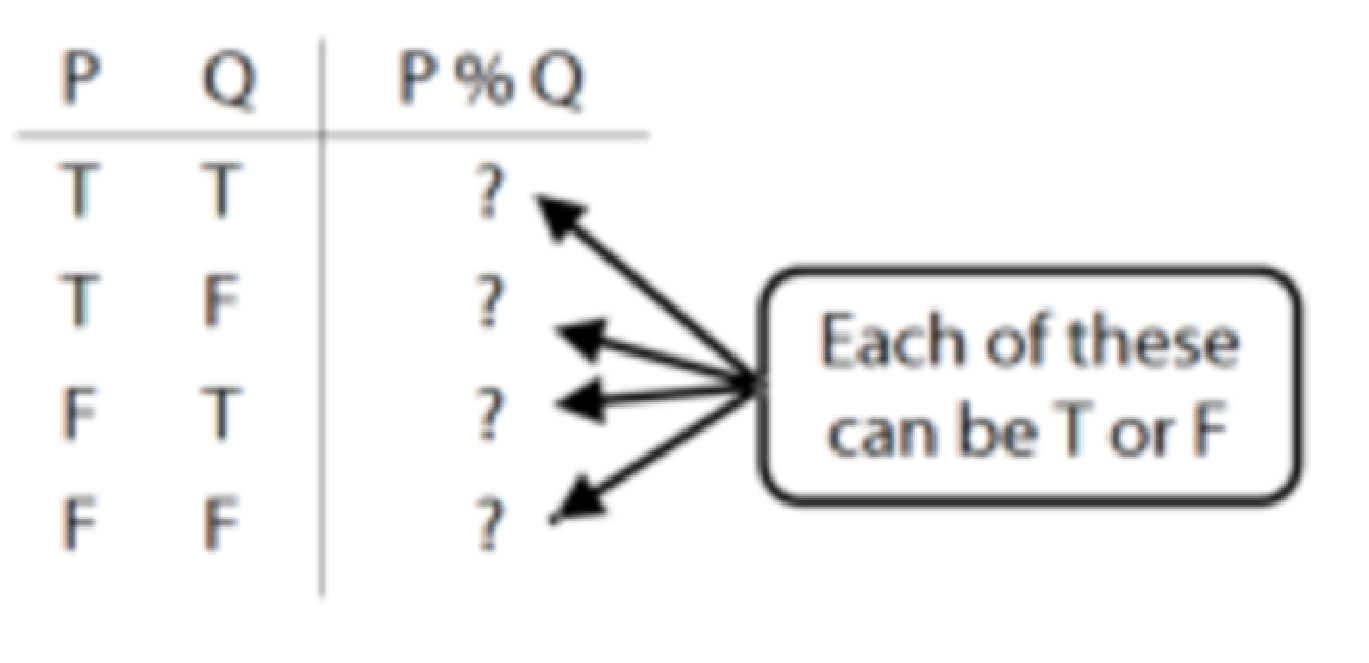
\includegraphics[scale=0.3]{img/unit_430_fig1.pdf}
\end{center}
 
 
\section{Truth-functional completeness}
 
\emph{Reading:} §7.4
 
‘A set of truth-functors is said to be \emph{expressively adequate} (or sometimes \emph{functionally complete}) iff, for every truth-function whatever, there is a formula containing only those truth-functors which express that truth-function, i.e. which has as its truth-table the truth-table specifying that function.’ (Bostock, \emph{Intermediate Logic} p. 45)
 
Illustration of the proof that $\{$¬, ∧, ∨$\}$ is truth-functionally complete:
 
\begin{center}
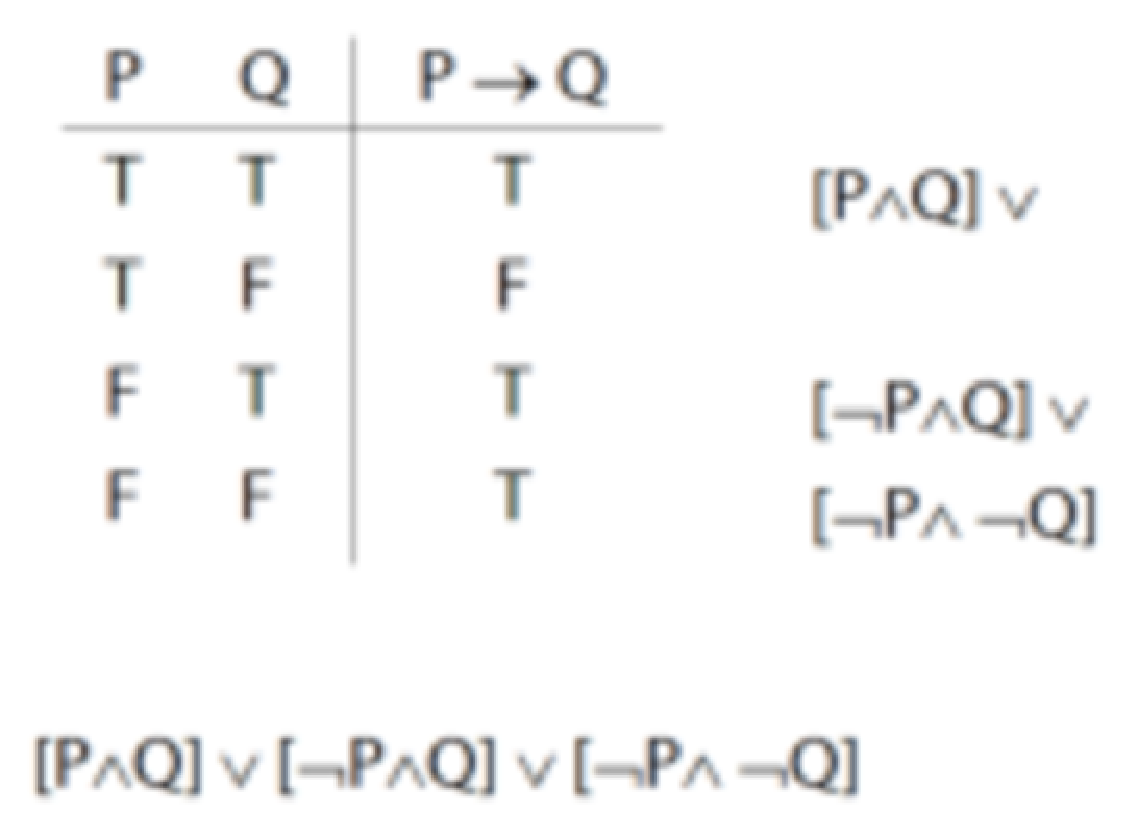
\includegraphics[scale=0.3]{img/unit_430_fig2.pdf}
\end{center}
\emph{Exercise} assuming $\{$¬,∨,∧$\}$ is truth-functionally complete, show that $\{$¬,∨$\}$ is.
 
 
 
\section{Soundness and Completeness: Statement of the Theorems}
 
\emph{Reading:} §8.3, §13.4
 
‘A $\vdash$ B’ means there is a proof of B using premises A
 
‘$\vdash$ B’ means there is a proof of B using no premises
 
‘A $\models$ B’ means B is a logical consequence of A
 
‘$\models$ B’ means B is a tautology
 
‘A $\models$$_{TT}$ B’ means B is a logical consequence of A just in virtue of the meanings of truth-functions (the textbook LPL calls this ‘tautological consequence’)
 
\emph{Soundness}: If A $\vdash$ B then A $\models$ B
 
\hspace{3mm} i.e. if you can prove it in Fitch, it’s valid
 
\emph{Completeness}: If A $\models$$_{TT}$ B then A $\vdash$ B
 
\hspace{3mm} i.e. if it’s valid just in virtue of the meanings of the truth-functional connectives, then you can prove it in Fitch.
 
\vfill
\begin{minipage}{\columnwidth}
\section{Exercises}
These exercises will be discussed in seminars the week after this lecture.
The numbers below refer to the numbered exercises in the course textbook, e.g.\ `1.1' refers to exercise 1.1. on page 39 of the second edition of \emph{Language, Proof and Logic}. Exercises marked `*' are optional.
 
\begin{quote}
13.12, 13.14, 13.16
 
13.43--13.45
 
13.49--13.50
 
9.18--9.19
 
11.10, 11.13
 
14.2
 
7.25, 7.26, *7.28, 7.29
 \end{quote}
\end{minipage}

%--- end paste
%--------------- 
 

\end{multicols*}

\end{document}